\HeaderQuote{I don't believe there's an atom of meaning in it.}{Alice}

\chapter{Analysing Solutions}\label{ch:analysingsol} 

\FirstSentence{I}{t is interesting to know if the difference} in the structure 
of the schedule is time dependent, e.g.,  is there a clear time of divergence 
within the scheduling process? 
Moreover, investigation of how sensitive is the difference between two sets of 
features, e.g., can two schedules with similar feature values yield 
\begin{enumerate*}[itemjoin={{? }}, itemjoin*={{? Or }}, after={{? }}]
    \item completely contradictory outcomes (i.e. one poor and one good 
    schedule)
    \item will they more or less follow the their predicted trend
\end{enumerate*}
If the latter is the prevalent case, then instances need to be segregated 
w.r.t. their difficulty, where each has their own learning algorithm 
implemented, for a more meaningful overall outcome.  

Essentially this also answers the question of whether  it is in fact feasible 
to discriminate between \emph{good} and \emph{bad} schedules using the 
currently selected features as a measure for the quality of a solution. 
If results are contradictory, then it is an indicator the features selected are 
not robust enough to capture the essence of the data structure and some key 
features are missing from the feature set that could be able to discriminate 
between \emph{good} and \emph{bad} schedules. 
Additionally, there is also the question of how to define `similar'
schedules, and what measures should be used? This 
\lcnamecref{ch:defdifficulty} describes some preliminary experiments with 
the aim of investigating the feasibility of finding distinguishing features 
corresponding to \emph{good} and \emph{bad} schedules in \jsp. To summarise
\begin{enumerate*}[itemjoin={{? }}, itemjoin*={{? And }}, after={{? }}]
    \item is there a time of divergence
    \item what are `similar' schedules
    \item do similar features yield contradictory outcomes
    \item are extra features needed
    \item what can be learned from feature behaviour
\end{enumerate*}

\emph{Remark:} \Cref{fig:diff:opt:unique,fig:diff:opt:rnd} 
depict the mean over all the training data, which are quite noisy 
functions. Thus, for clarity purposes, they are fitted with local polynomial 
regression, making the boundary points sometimes biased. 
\Cref{InRu15b} depicts the raw mean as is, albeit only for $10\times10$ problem 
spaces, which is also done here for 
\cref{fig:diff:extr:SDR,fig:diff:case:OPT,fig:diff:extr:features,fig:diff:extr:SDR,fig:diff:opt:evol}.

\section{Making optimal decisions}
In order to create successful \dr, a good starting point is 
to investigate the properties of optimal solutions and hopefully be able to 
learn how to mimic such `good' behaviour. 
For this, we follow an optimal solution (cf. $\Phi^\OPT$ in 
\cref{sec:trdat:tracks}),
and inspect the evolution of its features  (defined in \cref{tbl:features}) 
throughout the dispatching process, which is detailed in \cref{ch:gentrdat}. 
Moreover, it is noted, that there are several optimal solutions available for 
each problem instance. However, it is deemed sufficient to inspect only one 
optimal trajectory per problem instance as there are $N_{\train}$ 
independent instances which gives the training data variety. 

Firstly, we can observe that on a step-by-step basis there are several optimal 
dispatches to choose from. \Cref{fig:diff:opt:unique} depicts how the number of 
optimal dispatches evolve at each dispatch iteration. Note, that only one 
optimal trajectory is pursued (chosen at random), hence this is only a lower 
bound of uniqueness of optimal solutions.
As the number of possible dispatches decrease over time, 
\cref{fig:diff:opt:rnd} 
depicts the probability of choosing an optimal dispatch at each iteration. 

To generalise, we could consider the probability of optimality as a sort of 
stepwise `training accuracy.' Then for a given policy $\pi$, we'd formalise its 
optimality (yet still maintaining optimal trajectory) as, 
\begin{equation} \label{eq:tracc:opt}
    \xi^\star_{\pi} := \Exp[\pi_{\star}]{\pi_{\star} = \pi}
\end{equation}
that is to say the mean likelihood of our policy $\pi$ being equivalent to the 
expert policy $\pi_\star$, i.e., $Y^{\pi_\star}=Y^\pi$. Note, for 
$\xi^\star_\pi$ we 
only need $\{\Phi^{\pi_\star},\mathcal{Y}^{\pi_\star}\}$ from 
\cref{eq:trdat:metadata}
\begin{enumerate*}
    \item retrace $\pi_\star$ as done in \cref{pseudo:constructJSP}
    \item inspect if the job $J_{j^*}$ chosen by $\pi$ yields the same 
    $C_{\max}^{\pi_\star(\vchi^{j^*})}$ as the true optimum, 
    $C_{\max}^{\pi_\star}$
\end{enumerate*}

\begin{figure}
  \centering
  \subcaptionbox{$6\times5$\label{fig:diff:opt:unique:6x5}}{
    \includegraphics[width=\linewidth]{figures/{stepwise.6x5.OPT.unique}.pdf}}
  \\
  \subcaptionbox{$10\times10$\label{fig:diff:opt:unique:10x10}}{
    \includegraphics[width=\linewidth]{figures/{stepwise.10x10.OPT.unique}.pdf}}
  \caption[Number of unique optimal dispatches]{Number of unique optimal 
    dispatches (lower bound).}
  \label{fig:diff:opt:unique}
\end{figure}

\begin{figure}\centering
  \subcaptionbox{$6\times5$\label{fig:diff:opt:rnd:6x5}}{
    \includegraphics[width=\linewidth]{figures/{stepwise.6x5.OPT}.pdf}}
  \\
  \subcaptionbox{$10\times10$\label{fig:diff:opt:rnd:10x10}}{
    \includegraphics[width=\linewidth]{figures/{stepwise.10x10.OPT}.pdf}}
  \caption{Probability of choosing optimal move (at random)}
  \label{fig:diff:opt:rnd}
\end{figure}

\section{Making suboptimal decisions}\label{sec:diff:opt:sub}
Looking at \cref{fig:diff:opt:rnd}, \jrnd{10}{10} has a relatively high 
probability 
($70\%$ and above) of choosing an optimal job. However, it is imperative to 
keep making optimal decisions, because once off the optimal track the 
consequences can be dire. To demonstrate this interaction, 
\cref{fig:diff:case:OPT} 
depicts the worst and best case scenario of \namerho, once you've fallen off 
the optimal track, defined as follows,
\begin{subequations}\label{eq:bwc:opt}
  \begin{eqnarray} 
  \zeta_{\min}^{\star}(k) &:=& \Exp[\pi_\star]{\given{\min(\rho)}{
      \forall C_{\max}^{\vchi^j} \gneq C_{\max}^{\pi_\star} 
      \wedge J_j\in\mathcal{L}^{(k)} }} \\
  \zeta_{\max}^{\star}(k) &:=& \Exp[\pi_\star]{\given{\max(\rho)}{
      \forall C_{\max}^{\vchi^j} \gneq C_{\max}^{\pi_\star}
      \wedge J_j\in\mathcal{L}^{(k)} }}
  \end{eqnarray}
\end{subequations}
Note, that this is given that you make \emph{one} wrong 
turn. Generally, there will be many mistakes made, and then the compound 
effects of making suboptimal decisions really start adding up. 
In fact, \cref{fig:diff:extr:SDR} shows the probability of optimality when 
following a fixed SDR (i.e. if \cref{eq:tracc:opt} is conditioned on $\pi$ 
instead of $\pi_\star$).

It is interesting that for \JSP, then making suboptimal decisions makes more of 
an impact on the resulting makespan as the dispatching process progresses. 
This is most likely due to the fact that if a suboptimal decision is made in 
the early stages, then there is space to rectify the situation with the 
subsequent dispatches. 
However, if done at a later point in time, little is to be done as the damage 
has already been inflicted upon the schedule. 
However, for \FSP, the case is the exact opposite. Under those circumstances 
it's imperative to make good decisions right from the get-go. This is due to 
the major structural differences between \jsp\ and \fsp, namely the latter 
having a homogeneous machine ordering, constricting the solution immensely. 
Luckily, this does have the added benefit of making \fsp\ less vulnerable for 
suboptimal decisions later in the decision process. 

\begin{figure}\centering
  \subcaptionbox{$6\times5$\label{fig:diff:case:OPT:6x5}}{
    \includegraphics[width=\linewidth]{figures/ALL/{stepwise.6x5.OPT.casescenario}.pdf}\vspace*{-12pt}}
  \\
  \subcaptionbox{$10\times10$\label{fig:diff:case:OPT:10x10}}{
    \includegraphics[width=\linewidth]{figures/ALL/{stepwise.10x10.OPT.casescenario}.pdf}\vspace*{-12pt}}
  \caption[Mean \namerho, for best and worst case scenario for making one 
  suboptimal move]{Mean \namerho, for best and worst case scenario of when 
  making \emph{one} suboptimal dispatch (i.e. $\zeta_{\min}^{\star}$ and 
  $\zeta_{\max}^{\star}$), depicted as lower and upper bound, 
  respectively. Moreover, mean suboptimal move is given as dashed line.}
  \label{fig:diff:case:OPT}
\end{figure}


\section{Optimality of extremal features}\label{sec:diff:opt:ext}
The training accuracy from \cref{eq:tracc:opt} of the aforementioned 
features from \cref{tbl:features}, or probability of a job chosen by an 
extremal value for a feature being able to yield an optimal makespan on a 
step-by-step basis, i.e., $\xi^\star_{\pm\phi_i}$, 
is depicted in \cref{fig:diff:extr:features}, for both \jrnd{6}{5} and 
\jrnd{10}{10}.\footnote{Additional problem spaces for $\xi^\star_{\pm\phi_i}$
    can be found in \shiny: Features $>$ Extremal.}
Moreover, the dashed line represents the benchmark of randomly guessing the 
optimum, $\xi^\star_{\RND}$ (cf. \cref{fig:diff:opt:rnd}).
Furthermore, the \lcnamecref{fig:diff:extr:features}s are annotated with the 
corresponding mean \namerho, for the training set if it were scheduled solely 
w.r.t. that extremal feature.

Generally, a high stepwise optimality means a low $\rho$, e.g., 
\phiGlobalRelated, save for \phiRNDstd.\footnote{Note, \phiRNDstd\ is 
non-informative on its own, as a tight standard deviation implies either 
consistently high \emph{or} low $C_{\max}$ from the roll-outs.} 
Unfortunately, it's not always so predictable. Take for instance \phiproc, then 
the minimum value gives a better $\rho$, even though it's unlikelier to be 
optimal than it's maximum counterpart.

\clearpage
Before inspecting the local based features further. Notice that the staggering 
performance edge for \phiRNDmin\ is lost when going to a higher dimension (cf. 
\phiRNDmin\ in \cref{fig:diff:extr:jrnd:6x5} has $\rho=1.3\%$ and increases to 
8.8\% in  \cref{fig:diff:extr:jrnd:10x10}), implying that 100 random roll-outs 
for are not sufficient for fully exploring $10\times10$ state-space, yet highly 
competitive for $6\times5$.

\begin{figure}\centering
    \captionsetup{list=no}
    \subcaptionbox{\jrnd{6}{5}\label{fig:diff:extr:jrnd:6x5}}{
        \includegraphics[width=\linewidth]{figures/{j.rnd}/{stepwise.6x5.OPT.extremal}.pdf}}
    \caption{Probability of extremal feature being optimal}
    \label{fig:diff:extr:features}
\end{figure}
\begin{figure}\centering
    \captionsetup{list=no}
    \ContinuedFloat
    \subcaptionbox{\jrnd{10}{10}\label{fig:diff:extr:jrnd:10x10}}{
        \includegraphics[width=\linewidth]{figures/{j.rnd}/{stepwise.10x10.OPT.extremal}.pdf}}
    \caption{}
    \MyCaption{Probability of extremal feature being 
    optimal}{fig:diff:extr:jrnd:6x5}{fig:diff:extr:jrnd:10x10}
\end{figure}

\begin{figure}[p]\centering
  \captionsetup{list=no}
  \subcaptionbox{$6\times5$\label{fig:diff:extr:SDR:6x5}}{
    \includegraphics[width=\linewidth]{figures/{stepwise.6x5.SDR}.pdf}}
  \caption[Probability of SDR yielding optimal move]{
    Probability of SDR yielding optimal move. 
    Both optimal (solid: $\xi^\star_{\SDR}$) and SDR-based (dashed: 
    $\xi_{\SDR}$) trajectories are inspected.}
  \label{fig:diff:extr:SDR}
\end{figure}
\begin{figure}[p]\centering
  \captionsetup{list=no}
  \ContinuedFloat
  \subcaptionbox{$10\times10$\label{fig:diff:extr:SDR:10x10}}{
    \begin{tikzpicture}
    \node[anchor=south west,inner sep=0] (image) at (0,0,0) 
    {\includegraphics[width=\linewidth]{figures/{stepwise.10x10.SDR}.pdf}};
    \begin{scope}[x={(image.south east)},y={(image.north west)}]
    \node (zoom) at (0.27,.45)
    {\includegraphics[width=0.24\linewidth]{figures/j.rnd/{stepwise.10x10.SDR.zoom}.pdf}};
    \end{scope}
    \end{tikzpicture}\vspace*{-12pt}}
  \caption{Note, due to computational complexity, only \jrnd{10}{10} has 
    SDR-based trajectories also inspected. Otherwise, only optimal is pursued.}
  \MyCaption{Probability of SDR being optimal 
    move}{fig:diff:extr:SDR:6x5}{fig:diff:extr:SDR:10x10}
\end{figure}

\subsection*{Optimality of SDRs}
Let's limit ourselves to only features that correspond to SDRs from 
\cref{sec:SDR}. Namely, \cref{eq:CDR:SDR} yield
\begin{enumerate*}
    \item \phiproc\ for SPT and LPT
    \item \phijobWrm\ for LWR and MWR 
\end{enumerate*}
By choosing the lowest value for the first SDR, and highest value for the 
latter SDR, i.e., the extremal values for those given features. 
\Cref{fig:diff:extr:SDR} depicts the corresponding probabilities from 
\cref{fig:diff:extr:features} in one graph, for all problem spaces in 
\cref{tbl:data}.

Now, let's bare in mind \namerho, of applying SDRs throughout the dispatching 
process (cf. box-plots of which in \cref{fig:SDR:boxplot}), then there is a 
some correspondence between high probability of stepwise optimality and low 
$\rho$. Alas, this isn't always the case, for \jrnd{10}{10} 
$\xi^\star_{\SPT}$ always outperforms $\xi^\star_{\LPT}$ in 
choosing a 
dispatch which may result in an optimal schedule. However, this does not 
transcend to SPT having a lower $\rho$ value than LPT. Hence, it's not enough 
to just learn optimal behaviour, one needs to investigate what happens once we 
encounter suboptimal state spaces.

Since we know that our SDR heuristics aren't  perfect, and they're bound 
to make mistakes at some point. 
It's interesting to see how that stepwise optimality evolves for its intended 
trajectory, thereby updating \cref{eq:tracc:opt} to
\begin{equation} \label{eq:tracc:track}
    \xi_{\pi} := \Exp[\pi]{\pi_{\star} = \pi}
\end{equation}
\Cref{fig:diff:extr:SDR} shows the difference between $\xi^\star_{\SDR}$ and 
$\xi_{\SDR}$.
Similarly for \cref{eq:bwc:opt}, 
\begin{subequations}\label{eq:bwc:track}
\begin{IEEEeqnarray}{rCl}
  \zeta_{\min}^{\pi}(k) &:=& \Exp[\pi]{\given{\min(\rho)}{
      \forall C_{\max}^{\pi_\star(\vchi^{j})} \neq 
      C_{\max}^{\pi_\star(\vchi^{j^*})} \wedge j^* = 
      \argmax_{J_j\in\mathcal{L}^{(k)}}\{\pi(\vphi^j)\}
      }} \\
  \zeta_{\max}^{\pi}(k) &:=& \Exp[\pi]{\given{\max(\rho)}{
      \forall C_{\max}^{\pi_\star(\vchi^j)} \neq 
      C_{\max}^{\pi_\star(\vchi^{j^*})} \wedge j^* = 
      \argmax_{J_j\in\mathcal{L}^{(k)}}\{\pi(\vphi^j)\} 
      }} \\
  \zeta_{\mu}^{\pi}(k) &:=& \Exp[\pi]{\given{\rho}{
          C_{\max}^{\pi_\star(\vchi^{j^*})} \wedge j^* = 
          \argmax_{J_j\in\mathcal{L}^{(k)}}\{\pi(\vphi^j)\} 
      }} \label{eq:bwc:track:mu}
\end{IEEEeqnarray}
\end{subequations}
with the additional metric $\zeta_{\mu}^{\pi}$, which gives the mean evolution 
for \namerho, when following a fixed policy $\pi$.
Note, $\zeta^{\pi_{\star}}_{\min}=\zeta^{\star}_{\min}, 
\zeta^{\pi_{\star}}_{\max}=\zeta^{\star}_{\max}$ and 
$\zeta^{\pi_{\star}}_{\mu}=0$.
\Cref{fig:diff:case:SDR} depicts \cref{eq:bwc:track} for expert policy 
$\pi_\star$ and SDRs.

\begin{figure}[p]\centering
    \captionsetup{list=no}
    \subcaptionbox{$10\times10$\label{fig:diff:case:SDR:10x10}}{
        \includegraphics[width=0.8\linewidth]{figures/{j.rnd}/{stepwise.10x10.ALL.casescenario}.pdf}\vspace*{-12pt}}
    \caption{Mean \namerho, for best and worst case scenario when not
        following a fixed policy $\pi$ (i.e. $\zeta_{\min}^\pi$ and 
        $\zeta_{\max}^\pi$), depicted as lower and upper bound, respectively. 
        Moreover, mean evolution of $\rho$ for $\pi$ (i.e. $\zeta_{\mu}^{\pi}$) 
        is given as a dashed line.}
\end{figure}
\begin{figure}[p]\centering
    \captionsetup{list=no}
    \ContinuedFloat
    \subcaptionbox{$6\times5$\label{fig:diff:case:SDR:6x5}}{
        \includegraphics[width=\linewidth]{figures/ALL/{stepwise.6x5.ALL.casescenario}.pdf}}
    \caption{Note, $\{\zeta^{\pi^\star}_{\min},\zeta^{\pi^\star}_{\max}\}$ are 
    illustrated jointly for \Problem{\train} in \cref{fig:diff:case:OPT}}
    \MyCaption{Mean \namerho, for best and worst case scenario for not following
    a fixed policy}{fig:diff:case:SDR:10x10}{fig:diff:case:SDR:6x5}
    \label{fig:diff:case:SDR}
\end{figure}

\clearpage

A means of interpreting \cref{eq:bwc:track}, is that given a fixed policy 
$\pi$, then $\zeta_{\min}^{\pi}$ describes the potential improvement (iff 
$\zeta_{\min}^{\pi}<\zeta_{\mu}^{\pi}$) for changing the policy. Whereas, 
$\zeta_{\max}^{\pi}$ indicates the disadvantages of changing course. 
When $\zeta_{\min}^{\pi}>\zeta_{\mu}^{\pi}$, then clearly $\pi$ is not a good 
policy for said problem space, e.g., for the final dispatches of 
$\zeta_{\mu}^{\SPT}$ for \jrndJ{6}{5} or \jrnd{10}{10}. 

\emph{Remark}: \cref{eq:tracc:track,eq:bwc:track} are based on corresponding 
meta-data, $\{\Phi^\pi,\mathcal{Y}^\pi\}$ , from \cref{eq:trdat:metadata}, 
whereas \cref{eq:tracc:opt,eq:bwc:opt} reuse the same expert meta-data,
$\{\Phi^{\pi_\star},\mathcal{Y}^{\pi_\star}\}$.

\section{Simple blended dispatching rule}\label{sec:diff:opt:bdr}
The goal of this \lcnamecref{ch:defdifficulty} is to utilise feature behaviour 
to motivate new (and \emph{hopefully} better) \dr s. 
A na\"ive approach would be creating a simple blended \dr\ (BDR) which 
would be for instance switching between two SDRs at a predetermined time point. 

For instance, MWR and SPT hardly ever coincide for easy or hard schedules (cf. 
\cref{tbl:easy:cnt:10x10,tbl:hard:cnt:10x10}), so its reasonable to believe 
they could complement one another.
Going back to \cref{fig:diff:extr:SDR:10x10} a presumably good BDR for 
\jrnd{10}{10}  would be starting with $\xi^\star_{\SPT}(k)$ and then 
switching over to $\xi^\star_{\MWR}(k)$ at around time step $k=40$, where 
the SDRs change places in outperforming one another.
In addition, we can see that even though $\xi_{\SPT}(k)$ is generally 
more likely to find optimal dispatches in the initial steps, shortly after 
$k=15$ then $\xi_{\MWR}(k)$ becomes a contender again. 
A box-plot of \namerho, for \Problem[10\times10]{\train} is 
depicted in \cref{fig:diff:boxplot:BDR} for a switch between SPT to MWR at time 
steps $k=\{10,15,20,30,40\}$. Main statistics are given in \cref{tbl:BDR:stats}.

This little manipulation between SDRs does outperform SPT immensely, yet 
doesn't manage to gain the performance edge of MWR. 
This gives us insight that for \jsp, the attribute based on MWR is quite 
fruitful for good dispatches, whereas the same cannot be said about SPT -- a 
more sophisticated DR is needed to improve upon MWR. 

A reason for this lack of performance of our proposed BDR at $k=40$ is perhaps 
that by starting out with SPT in the beginning, it sets up the schedules in 
such a way that it's quite greedy and only takes into consideration jobs with 
shortest immediate processing times. 
Now, even though it is possible to find optimal schedules from this scenario, 
as \cref{fig:diff:extr:SDR} shows, the inherent structure is already taking 
place, and might make it hard to come across optimal moves by simple methods. 
Therefore it's by no means guaranteed that by simply swapping over to MWR will 
handle the situation that applying SPT has already created. 
\Cref{fig:diff:boxplot:BDR} does however show, that by applying MWR instead of 
SPT in the latter stages, does help the schedule to be more compact w.r.t. SPT. 
However, the fact remains that the schedules have diverged too far from what 
MWR would have been able to achieve on its own, i.e., using SPT downgrades the 
performance of MWR. 

Changing to MWR at $k\leq20$ is not statically significant from MWR (boost in 
mean $\rho$ is at most 0.5\%). 
However, after $k>20$ then the BDR starts diverging from MWR. 
But as pointed in \cref{sec:diff:opt:sub}, it's not so fatal to make bad moves 
in the very first dispatches for \jrnd{10}{10}, hence little is gained with 
improved classification accuracy in that region. 
But this does tell us that $\xi_\pi$ is a more reliable indicator than 
$\xi^\star_\pi$ when it comes to choosing appropriate model parameters. 
Alas, $\xi_\pi$ requires collecting the meta-data 
$\{\Phi^\pi,\mathcal{Y}^\pi\}$ from \cref{eq:trdat:metadata} for its policy 
$\pi$, whereas $\xi^\star_\pi$ reuses 
$\{\Phi^{\pi_\star},\mathcal{Y}^{\pi_\star}\}$ 
for each new policy $\pi$.

Revisiting \cref{fig:diff:case:SDR:10x10}, then we see 
$\zeta_{\mu}^{\SPT}(40)$ has already surpassed 
$\zeta_{\mu}^{\MWR}(K)$ and there are 60 operations left to dispatch. So 
a switch for BDR at $k=40$ never had a chance of improvement. 
However, at $k\leq15$ then $\zeta_{\mu}^{\SPT}(k) < 
\zeta_{\mu}^{\MWR}(k)$, which were appropriate turning points for BDR 
(although not statistically significant).

Preferably the blended dispatching rule should use best of both worlds, and 
outperform all of its inherited DRs, otherwise it goes without saying, one 
would simply keep on still using the original DR that achieved the best results.

\begin{figure}[p]
  \centering
  \includegraphics[width=\linewidth]{figures/{j.rnd}/{boxplotRho.BDR.10x10}.pdf}
  \vspace*{-24pt}
  \caption{Box plot of \jrnd{10}{10} \namerho, for BDR where SPT is applied for 
  the first 10\%, 15\%, 20\%, 30\% or 40\% of the dispatches, followed by MWR.}
  \label{fig:diff:boxplot:BDR}
\end{figure}

\begin{table}[b]
\caption{Main statistics for \jrnd{10}{10} \namerho, using BDR that changes 
from SDR at a fixed time step $k$.}\label{tbl:BDR:stats} 
\centering
\begin{tabular}{ccrlrrrrrr}
  \toprule
  SDR \#1 & SDR \#2 & $k$ & Set & Min. & 1st Qu. & Median & Mean & 
    3rd Qu. & Max. \\ \midrule
  SPT & -- & $K$ & train & 20.38 & 41.15 & 50.70 & 51.31 & 59.18 & 94.20 \\ 
  SPT & -- & $K$ & test & 22.75 & 41.39 & 49.53 & 50.52 & 58.60 & 93.03 \\ 
  MWR & -- & $K$ & train & \textbf{4.42} & \textbf{17.84} & \textbf{21.74} & 
  22.13 & 26.00 & 47.78 \\ 
  MWR & -- & $K$ & test & \textbf{3.37} & \textbf{17.07} & 21.39 & 21.65 & 
  25.98 & \textbf{41.80} \\ 
  SPT & MWR & 10 & train & 5.54 & 17.98 & 21.75 & \textbf{21.99} & 
  \textbf{25.43} & \textbf{44.02} \\ 
  SPT & MWR & 10 & test & 5.87 & 17.29 & \textbf{20.78} & \textbf{21.28} & 
  \textbf{24.67} & 44.47 \\ 
  SPT & MWR & 15 & train & 4.76 & 18.24 & 22.04 & 22.49 & 26.65 & 49.86 \\ 
  SPT & MWR & 15 & test & 7.42 & 17.60 & 21.38 & 21.83 & 25.45 & 45.98 \\ 
  SPT & MWR & 20 & train & 5.76 & 18.98 & 22.46 & 23.01 & 26.97 & 41.59 \\ 
  SPT & MWR & 20 & test & 8.31 & 18.64 & 22.92 & 23.29 & 27.10 & 49.93 \\ 
  SPT & MWR & 30 & train & 9.77 & 20.89 & 25.60 & 25.76 & 30.01 & 50.94 \\ 
  SPT & MWR & 30 & test & 4.39 & 21.20 & 26.08 & 26.25 & 30.58 & 49.88 \\ 
  SPT & MWR & 40 & train & 13.04 & 23.42 & 28.12 & 28.94 & 33.67 & 54.98 \\ 
  SPT & MWR & 40 & test & 8.55 & 24.20 & 28.16 & 28.98 & 33.20 & 57.21 \\ 
  \bottomrule
\end{tabular}
\end{table}

\section{Feature evolution}\label{sec:diff:opt:evol}
In order to put the extremal features from \cref{fig:diff:extr:features} into 
perspective, it's worth comparing them with how the evolution of the features 
are over time, depicted in \cref{fig:diff:opt:evol} for \jrnd{6}{5} and 
\jrnd{10}{10}.\footnote{Additional problem spaces can be found in \shiny: 
    Features $>$ Evolution.} 
Note that the optimal trajectory describes  how `good' features should aspire 
to be like.
We can also notice that the relative ranking in \phiGlobalRelated\ is 
proportional their expected mean \namerho\ (i.e. $\zeta_{\mu}^{\pi}(K)$). 
Although $(K-k)$-step lookahead give consistently the best (single) indicators 
for finding good solutions. 
Sadly, they are not practical features for high dimensional data due to 
computational cost. 
Nevertheless, bearing \cref{fig:diff:case:OPT:10x10} in mind then it 
might be sufficient to do only a few steps lookahead at some key times in the 
dispatching process. For instance, let the computational budget for 
\frnd{10}{10} roll-outs be full $K$-solutions in the beginning phases, as 
that's when the problem space is most susceptible to bad moves. Then gradually 
decrease to only a few step lookahead, as \fsp\ is then relatively stable.
Conversely for \jrnd{10}{10}, start with a few step lookahead, and then 
expand the horizon as time goes by. Alternatively, when there aren't that many 
dispatches left, it might be worth developing a hybrid approach where the 
remaining dispatches from that point are optimised with some exact methods. 

\begin{figure}\centering
  \captionsetup{list=no}
  \subcaptionbox{\jrnd{6}{5}\label{diff:evol:jrnd:6x5}}{
    \includegraphics[width=\linewidth]{figures/{j.rnd}/{stepwise.6x5.evolution}.pdf}}
  \caption{Mean stepwise evolution of $\tilde{\vphi}$, which is scaled 
  according to \cref{eq:scale}}
  \label{fig:diff:opt:evol}
\end{figure}
\begin{figure}\centering
  \captionsetup{list=no}
  \ContinuedFloat
  \subcaptionbox{\jrnd{10}{10}\label{diff:evol:jrnd:10x10}}{
    \includegraphics[width=\linewidth]{figures/{j.rnd}/{stepwise.10x10.evolution}.pdf}}
  \caption{}
  \MyCaption{Mean stepwise evolution of 
  $\tilde{\vphi}$}{diff:evol:jrnd:6x5}{diff:evol:jrnd:10x10}
\end{figure}

\section{Emergence of problem difficulty}\label{sec:diff:stepwise}

% Katie orðar: A correlation analysis between the feature space and the 
%performance space was conducted across all 1,500 problem instances revealed 
%that instance features that appear to correlate (linearly) with heuristic 
%performance are $phi(?)$ (correlation $=-0.59$) and $phi(?)$ (correlation 
%$=0.44$). None of the other instance features appear to have a linear 
%relationship with algorithmic performance.

The main focus now is on knowing \emph{when} during the scheduling process easy 
and hard problems (using the difficulty definition from \cref{eq:easy.vs.hard}) 
diverge and explore in further detail \emph{why} they diverged. The number of 
segregated problem instances for \PhiSet{ALL} and 
$\Phi^{\SDR}$ (conditioned on the followed trajectory) for \jrnd{6}{5} are 
given in \cref{tbl:jrnd:feat:cnt}.\footnote{Additional problem spaces can be
     found in \shiny: Footprints $>$ Stepwise.} 

Rather than visualising high-dimensional data projected onto two dimensional 
space (as was the focus in \cite{SmithMilesLion5} with SOM), 
instead appropriate statistical tests with a significance level $\alpha=0.05$ 
is applied to determine if there is any difference between different data 
distributions. 
For this the two-sample Kolmogorov–Smirnov test (K-S test) is used to determine 
whether two underlying one-dimensional probability distributions differ. 
Furthermore, in order to find defining characteristics for easy or hard 
problems, a (linear) correlation is computed between features to the resulting 
\namerho\ and use a $t$-test for testing the population correlation 
coefficient. 

Note, when inspecting any statistical difference between data distribution of 
the features on a step-by-step basis, the features at step $k+1$ are of course 
dependant on all previous $k$ steps. This results in repetitive statistical 
testing, therefore a Bonferroni adjustment is used to counteract the multiple 
comparisons, i.e., each stepwise comparison has the significant level 
$\alpha_k=\frac{\alpha}{K}$, and thus maintaining the 
$\sum_{k=1}^K\alpha_k=\alpha$ significance level.

{\setlength{\tabcolsep}{3pt} 
\begin{table}\centering
    \caption{Number of problem instances after segregating \jrnd{6}{5} w.r.t. 
    difficulty and trajectory.}
    \label{tbl:jrnd:feat:cnt}
    \subcaptionbox{Used in \cref{fig:jrnd:feat:KStest}}{
        \begin{tabular}{lrrr}
            \toprule
            Track & $\#$Easy & $\#$Hard & $\#$Significant \\ 
            \midrule
            SPT &  37 & 203 &  48 \\ 
            LPT & 103 &  81 &  47 \\ 
            LWR &  19 & 295 &  31 \\ 
            MWR & 328 &   1 &   0 \\ 
            \midrule
             $\Sigma$ & 487 & 580 & 126 \\
             \bottomrule
        \end{tabular}
    }\quad\quad
    \subcaptionbox{Used in \cref{fig:jrnd:feat:corr}}{
        \begin{tabular}{lrr}
            \toprule
            & \multicolumn{2}{c}{$\#$Significant} \\
            Track & Easy & Hard \\ 
            \midrule
            SPT &  78 & 101 \\ 
            LPT &  87 &  45 \\ 
            LWR &  48 &  82 \\ 
            MWR & 167 &   0 \\ 
            ALL & 260 & 138 \\ 
            \midrule
            $\Sigma$ & 640 & 366 \\
            \bottomrule
        \end{tabular}}
\end{table}}

\begin{figure}[t]
    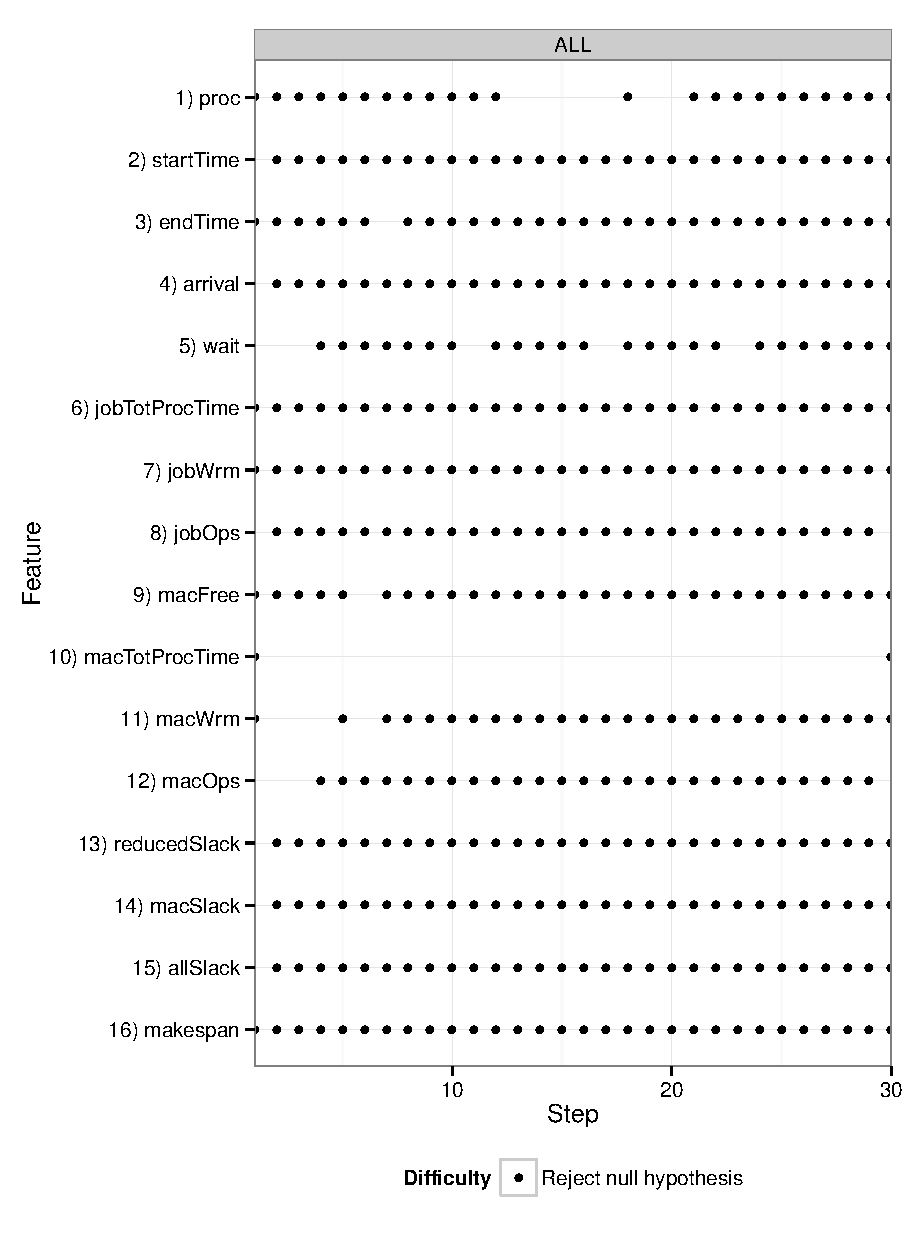
\includegraphics[width=\linewidth]{{j.rnd/phi.ks.SDR.6x5}.pdf}
    \caption{Stepwise K-S Test for features $\vphi$ segregated w.r.t. easy and 
        hard problems are drawn from the same data distribution.}
    \label{fig:jrnd:feat:KStest}
\end{figure}

\begin{figure}
    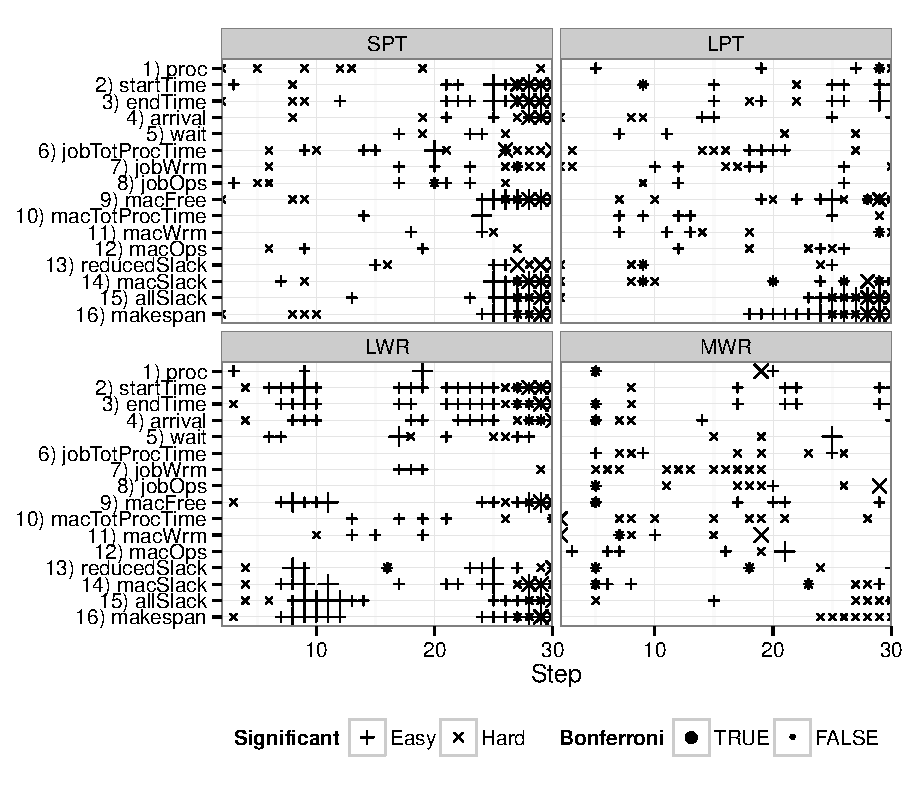
\includegraphics[width=\linewidth]{{j.rnd/phi.corr.SDR.6x5}.pdf}
    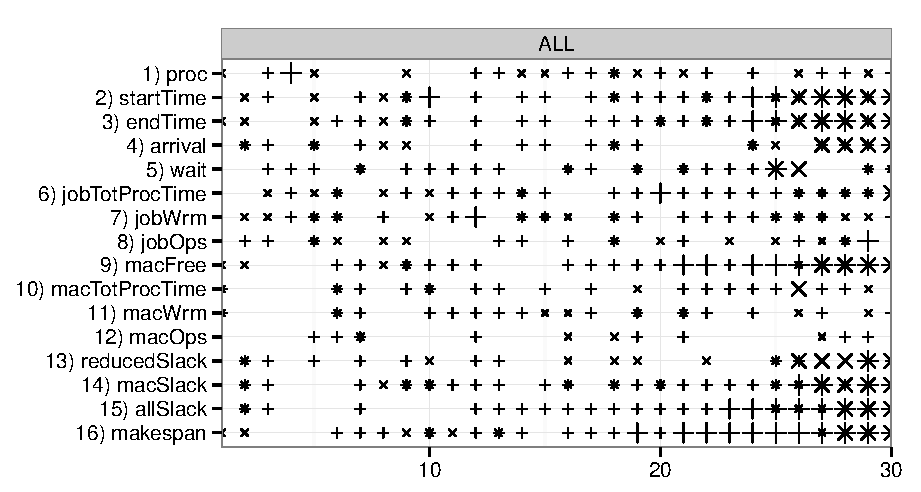
\includegraphics[width=\linewidth]{{j.rnd/phi.corr.ALL.6x5}.pdf}
    \caption{Stepwise significance of a correlation coefficient for \jrnd{6}{5} 
        features $\vphi$, segregated w.r.t. easy and hard problems, with 
        resulting 
        \namerho.}
    \label{fig:jrnd:feat:corr}
\end{figure}

\Cref{fig:jrnd:feat:KStest} indicates the timesteps when easy and hard feature 
distributions differ. In the initial stages, the features are more or less the 
same. However, there is a clear time of divergence towards the end of the 
scheduling process, around $k=25$ (little sooner for LPT and later for LWR).
\todoExtend{\cref{fig:jrnd:feat:KStest}}

Furthermore, \cref{fig:jrnd:feat:corr} shows when easy or hard features 
are significantly correlated to the \namerho.
There we can see an apparent difference in correlation between individual 
features with the resulting schedule depending in what stage it is in the 
scheduling process, implying that their influence varies over the dispatching 
sequencing. 
\todoExtend{\cref{fig:jrnd:feat:corr}}
There are some common features for both difficulties considered which define 
\jsp\ on a whole. However, the significant features are quite different across 
the two difficulties, implying there is a clear difference in their data 
structure. The amount of significant features were considerably more for easy 
problems, indicating their key elements had been found. However, the features 
distinguishing hard problems were scarce. Most likely due to their more complex 
data structure their key features are of a more composite nature. As a result, 
new `global' features were introduced. 

It is possible for a \JSP\ schedule to have more than one sequential 
dispatching representation. It is especially w.r.t. the initial dispatches. 
Revisiting \cref{fig:example:midway}, if we were to dispatch $J_2$ f
first and then $J_4$, then that would be the same equivalent
temporal schedule if we did it the other way around. 
This is because they don't create a conflict for one another 
(as is the case for jobs $J_2$ and $J_3$). This drawback of non-uniqueness of 
sequential dispatching representation explains why there is hardly any 
significant difference between the difficulties for the initial steps of the 
scheduling process (cf. \cref{fig:jrnd:feat:KStest}).
As we can see from \cref{tbl:jrnd:feat:cnt}, the number of problem instances 
used for statistical testing is quite limited when applying on a single 
algorithm. 
Using the non-uniqueness of $\vchi$ to our advantage, where there are many jobs 
that have non-conflicting machines, thereby making subsequent dispatches 
equivalent to the previous one, i.e., $\vchi^k \approx  \vchi^{(k\pm1)}$. 
Therefore it's reasonable, when labelled optimal data is scarce, to inspect the 
stepwise statistical testing based on sliding window of the preceding and 
subsequent step, i.e., test at time $k$ is based on: 
\begin{equation}
\vphi_i^{(k)} := \condset{\phi_i^{k'}}{\forall \phi_i\in\Phi}_{k'=k-1}^{k+1} 
\end{equation}
for all individual local features $\phi_i\in\{1,\ldots,\NrFeatLocal\}$ from 
\cref{tbl:features}.


\section{Summary and conclusions}

\todoWrite{From \cref{sec:diff:opt:ext} we noticed that high stepwise 
optimality generally implies low \namerho. Moreover, there is clearly an 
important factor \emph{when} suboptimal moves are made, as 
\cref{sec:diff:opt:sub} showed. Therefore it's not 
    }

Since feature selection is of paramount importance in order for algorithms to 
become successful, one needs to give great thought to how features are 
selected. What kind of features yield \emph{bad} schedules? And can they be 
steered onto the path of more promising feature characteristics? This sort of 
investigation can be an indicator how to create meaningful problem generators. 
On the account that real-world problem instances are scarce, their hidden 
properties need be drawn forth in order to generate artificial problem 
instances from the same data distribution. 

The feature attributes need to be based on statistical or theoretical grounds. 
Scrutiny in understanding the nature of problem instances therefore becomes of 
paramount importance in feature engineering for learning, as it yields feedback 
into what features are important to devote more attention to, i.e., features 
that result in a failing algorithm. 
For instance, in \cref{tbl:jrnd:feat:same} the slack features have the same 
distribution in the initial stages of the scheduling process. However, there is 
a clear point of divergence which needs to be investigate why the sudden 
change? \todoFind{Check with best/worst case scenario}
In general, this sort of analysis can undoubtedly be used in better 
algorithm design which is more equipped to deal with varying problem instances 
and tailor to individual problem instance's needs, i.e., a footprint-oriented 
algorithm.

Although this methodology was only implemented on a set of simple 
single-priority \dr s, the methodology is easily adaptable for more 
complex algorithms, such as the learned preference models in 
\cref{ch:prefmodels}. The main objective of this work is to 
illustrate the interaction of a specific algorithm on a given problem structure 
and its properties. 

\todoWrite{
  In this \lcnamecref{ch:defdifficulty} we will find the footprint 
  from \sdr s introduced in \cref{sec:SDR} on those problem spaces. Presumably, 
  we could use that information to infer the complexity of our synthesised 
  problem spaces summarised in \cref{tbl:data}.}
